%!TEX root = ../notas_de_clase.tex

\section{Aprendizaje No Supervisado}

\subsection{Reducción de dimensionalidad}
\subsubsection{Análisis de componentes principales (ACP)}

Consideremos un conjunto de observaciones de $\{\x_i\}_{i=1}^n\subset\R^N$, donde denotamos $\x_i=[x_{i1},x_{i2},\ldots,x_{iN}]^\top$. Podemos entender que el elemento $x_{ij}$ corresponde al valor del atributo $j$ para la observación $i$. 

\begin{mdframed}[style=pendiente, frametitle={\center ejemplos}]
dar un ejemplo como el de nutrición, series de tiempo, geo-algo
\end{mdframed}

Notemos que cada observación puede descomponerse en la base canónica $\{\e_i\}_{i=1}^N$ de $\R^N$ de la forma 
\begin{equation}
	\x_i = x_{i1}\e_1 +  x_{i2}\e_2 + \cdots + x_{iN}\e_N 		
\end{equation}
Notemos que es posible representar cada vector $\x_i$ mediante una cantidad $N'<N$ de términos truncando la representación anterior, es decir,  
\begin{equation}
	\x_i \approx \sum_{j=1}^{N'} x_{i\sigma(j)}\e_{\sigma(j)}
\end{equation}
donde $\sigma:\{1,2,\ldots,N\}\mapsto\{1,2,\ldots,N\}$ es una permutación. Dicha aproximación de las observaciones $\{\x_i\}_{i=1}^n$ es una versión de baja dimensión, entonces, naturalmente nos podemos hacer la siguiente pregunta: dado una dimensión $N'<N$  ¿es efectivamente un subconjunto de los vectores canónicos la mejor base para descomponer as observaciones?  ¿cómo encontramos la \emph{mejor} base?

La respuesta a la primera pregunta es, en la mayoría de los casos, negativa. Esto es porque los elementos de la base canónica, por sí solos, conllevan poca información estructural que puede ser encontrada en los vectores observados. En particular, consideremos el caso en donde solo se dispone de dos observaciones $\{\x_1, \x_2\}$, si $N'=2$, entonces una descomposición que garantiza error nulo es simplemente elegir $\x_1$ y $\x_2$ como bases de la nueva descomposición, donde los coeficientes estarían dados por $[1,\ 0]^\top$ y $[0,\ 1]^\top$. 

Para encontrar la \emph{mejor} base, lo primero que se requiere es definir qué se entiende por \emph{mejor}. Nos enfocaremos en determinar una base cuyos componentes \textbf{ordenados} $\cvector_1,\cvector_2,\ldots$ capturan las $N'$ direcciones (ortogonales) de máxima variabilidad de nuestros datos. Es decir, el primer elemento de la nueva base estará dado por 
\begin{equation}
	\cvector_1 = \argmax_{||\cvector_1||=1} {\langle\cvector_1,\x\rangle} \label{eq:PCA_max}
\end{equation}
Este criterio es conocido como \textbf{análisis de componentes principales (ACP)}. Notemos que la restricción $||\cvector_1||=1$ es porque recordemos que estamos la dirección de máxima varianza y  la expresión anterior (cuadrática en $\cvector_1$) no es maximizable en $\cvector_1$. Por esta razón, sin pérdida de generalidad podemos fijar la norma de $\cvector_1$ en 1 y buscar una base \emph{ortonormal}. 

Asumiremos además que nuestros datos están estandarizados, es decir, tienen un vector de medias nulo y varianzas marginales unitarias. Esto es para reducir los sesgos por variables que pueden ser introducidos en la maximización de la expresión anterior: Si una dimensión tiene una varianza marginal mayor que el resto, ésta será más importante en la determinación de la dirección de máxima varianza solo por su magnitud y no por la relación entre variables. 

Como en general no contamos con la distribución de las observaciones $p(\x)$, podemos considerar una aproximación muestral de la varianza en la ecuación \eqref{eq:PCA_max} y resolver 
\begin{align}
	\cvector_1 = \argmax_{||\cvector_1||=1} \sum_{i=1}^N \langle\cvector_1,\x\rangle^2.\label{eq:PCA_max2}
\end{align}

Podemos ahora usar la siguiente notación
$$
X=[\x_1,\x_2,\ldots,,\x_n]=\begin{bmatrix}
        {x}_{11}    & \dots & {x}_{n1}  \\
        \cdots          & \ddots& \cdots        \\
        {x}_{1N}    & \dots & {x}_{nN}
        \end{bmatrix},
$$
y reescribir la ecuación \eqref{eq:PCA_max2} como 
\begin{align}
	\cvector_1 = \argmax_{||\cvector_1||=1} ||\cvector_1^\top X||^2 
			= \argmax_{||\cvector_1||=1} \cvector_1^\top XX^\top \cvector_1
			= \argmax_{\cvector_1} \frac{\cvector_1^\top XX^\top \cvector_1}{\cvector_1^\top \cvector_1}. 
			\label{eq:PCA_max3}
\end{align}
donde la última igualdad incorpora la normalización de $\cvector_1$ la cual permite formular el problema de optimización irrestricto. La expresión de la derecha se llama cuociente de Rayleigh para la matriz simétrica $XX^\top$, donde sabemos que la maximización de este cuociente está dado por el vector propio de la matriz $XX^\top$ asociado al mayor valor propio. Observe que $XX^\top$ es la matriz de correlación muestreal del conjunto de observaciones $\{\x_i\}_{i=1}^n$, consecuentemente, la proyección de una observación $\x_i$ en la dirección de máxima varianza, o bien la \emph{primera componente principal}, está dada por 
\begin{equation}
	\x_i^{(1)} = \langle \x_i, \cvector_1 \rangle
\end{equation}
donde $\cvector_1$ es el vector propio asociado al mayor valor propio de la matriz de covarianza muestreal $XX^\top$.

El cálculo de las siguientes componentes se realiza de forma iterativa sobre los residuos del conjunto de observaciones con respecto a las componentes anteriores. De esta forma, ACP encuentra una nueva base ortonormal tal que las componentes maximicen la variabilidad donde en algunos casos se puede perder intepretabilidad de las nuevas características generadas, pues son combinaciones lineales de las características originales de los datos. A pesar de esto, utilizando las primeras 2 o 3 componentes PCA se pueden visualizar datos de alta dimensionabilidad de forma ilustrativa.


\subsubsection{Kernel PCA}
El método Kernel PCA es similar a PCA, pero esta vez se utiliza el truco del kernel para proyectar los datos. En ese sentido, en vez de calcular la matriz de covarianza empírica, se utiliza la matriz de Gram.

$$
K_{ij} = K(x_i,x_j) = \phi(x_i)\phi(x_j)^T
$$

Luego, se prosigue de la misma forma que PCA linear.

En la figura \ref{fig:kpca} se puede observar un ejemplo en que el resultado de PCA linear no es suficiente, puesto que el problema es simétrico, mientras que KPCA realiza una correcta separación de ambos clusters.

\begin{figure}[ht]
    \centering
    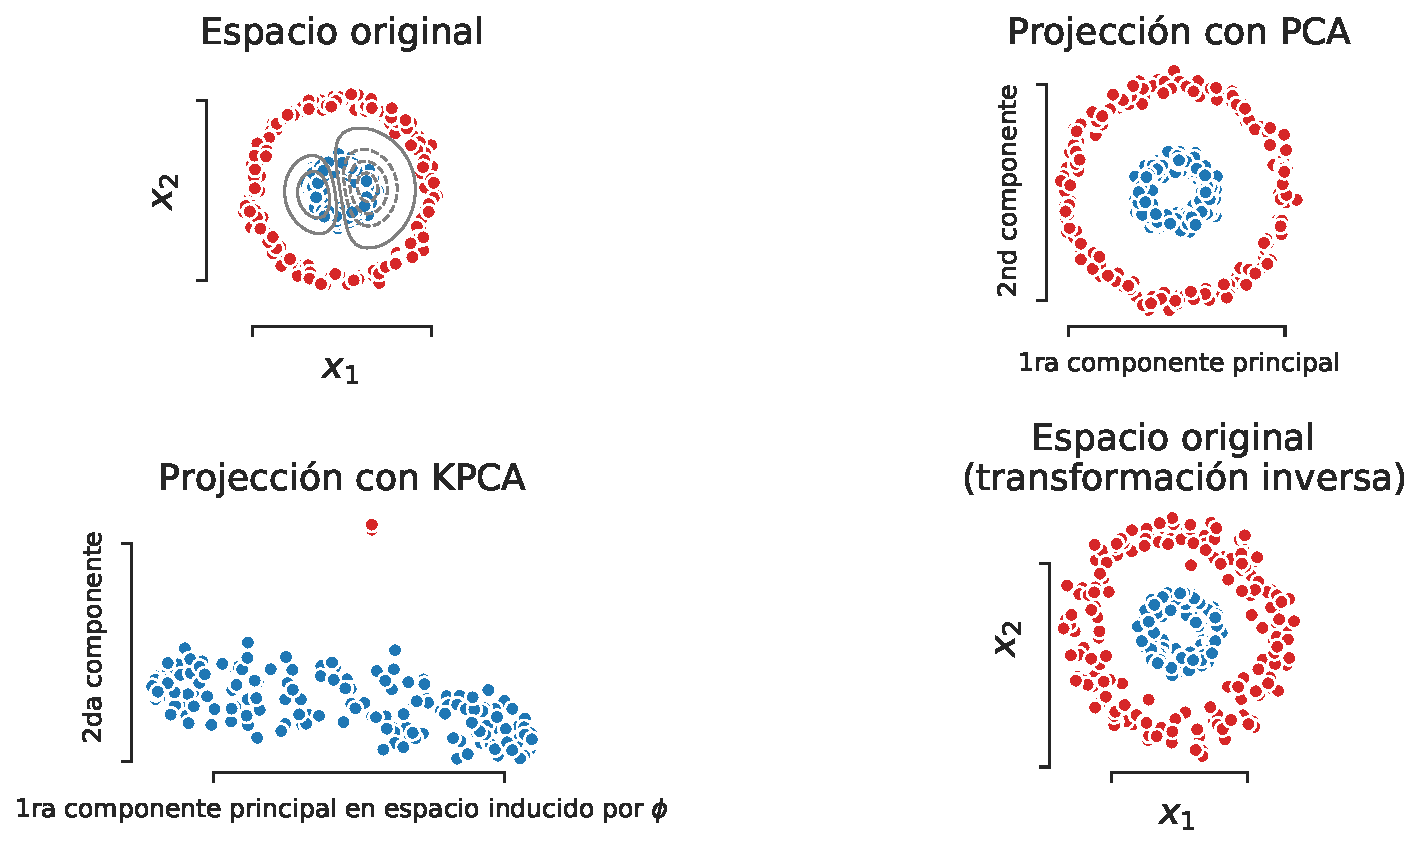
\includegraphics[width=0.7\linewidth]{img/cap7_kpca.pdf}
    \caption{Ejemplo en que kernel PCA sobre un conjunto de datos que no es linealmente separable.}
    \label{fig:kpca}
\end{figure}

\subsubsection{Probabilistic PCA}
PCA probabilístico (PPCA, por su sigla en inglés) tiene su inspiración en que PCA se puede expresar como la solución via máxima verosimilitud de un modelo probabilístico de variable latente. De este modo, PPCA propone un método iterativo para obtener la solución evaluando solo cierto número de componentes, sin necesidad de calcular la matriz de covarianza empírica.

El modelo probabilístico para PCA en que se inspira PPCA es el siguiente:

Sea $x_i\in \mathbb{R}^m$ los elementos observados, inputs o variables y $z\in \mathbb{R}^l$ una variable latente explícita correspondiente al espacio de las componentes principales. Se define un prior para $z$:

\begin{equation}
p(z) = N(0,I)
\end{equation}

De este modo, la distribución condicional de x dado z también es Gaussiana:

\begin{equation}
p(x|z) = N(Wz+\mu,\sigma^2I)
\end{equation}
Donde $W\in \mathbb{R}^{M\times l}$ y $\mu \in \mathbb{R}^m$ son parámetros a determinar. Notemos que no se pierde generalidad tomar el prior para $z$ con media cero y varianza unitaria, puesto que si se toma otro prior más general, se produce el mismo modelo.

Dado que tenemos modelo paramétrico probabilístico, podemos estimar los parámetros con máxima verosimilitud. Dado los datos $X = \{x_i\}_{i=1}^n$. La log-verosimilitud está dada por:

\begin{align}
\log p(X|W,\mu, \sigma^2) & = \sum_{i=1}^n \log p(x_i|W,\mu, \sigma^2)\\
& = \frac{n l}{2}\log (2\pi) - \frac{n}{2}log|C| - \frac{1}{2}\sum_{i=1}^n (x_i-\mu)^T C^{-1} (x_i-\mu),
\end{align}

con $C = WW^T + \sigma^2 I$.

Usando la condición de primer orden obtenemos

\begin{align}
\mu = \bar{x} = \frac{1}{n}\sum_{i=1}^n x_i.
\end{align}
De esta manera tenemos la función de log-verosimilitud completa:

\begin{align}
    \log p(X, Z|W, \mu, \sigma^2) = \sum_{i=1}^n \{\log p(x_i|z_i) + \log p(z_i)\}
\end{align}

y evaluando en $\mu = \bar{x}$

\begin{align}
\notag \mathbb{E}[ p(X,Z |W, \mu, \sigma^2) ] =  -\sum_{i=1}^n \Bigg\{ &\frac{l}{2} \log (2\pi \sigma^2)\\
\notag & + \frac{1}{2}\text{Tr}(\mathbb{E}[z_iz_i^T])\\
\notag & \frac{1}{2\sigma^2}||x_i - \mu||^2 - \frac{1}{\sigma^2}\mathbb{E}[z_i]^T W^T (x_i - \mu)\\
& \frac{1}{2\sigma^2} \text{Tr}(\mathbb{E}[z_iz_i^T]W^T W) \Bigg\}
\end{align}



\section{Clustering}

\subsection{k-means}
Dado un entero $k \in \mathbb{N}$ y uin conjunto de observaciones $X = \{x_i\}_{i=1}$ con $x_i\in \mathbb{R}^D$ queremos separar los datos en k graupos, donde cada grupo se le asigna un centroide $\mu_k$ y cada elemento $x_i$ se le asigna el grupo que tenga el centroide más cercano.

Sea $r_{ik}$ la asignación, esta estará definida por:

\begin{align*}
r_{ik} = \begin{cases}
1 & \text{si } k = \text{argmin}||x_i-x_k||\\
0 & \text{si no.}
\end{cases}
\end{align*}
Es decir, para encontrar los centroides se debe minimizar la función:

\begin{align}
J = \sum_{i=1}^N \sum_{k=1}^K r_{ik} ||x_i-x_j||^2
\end{align}

Para minimizar esta función utilizaremos un enfoque llamado \emph{Expectation-Maximization}. Este es un método iterativo y como tal, tiene problemas con mínimo locales, pero para solucionar esto, basta inicializar el algoritmo muchas veces.

El algoritmo está dado por:

\begin{itemize}
    \item \textbf{E-step:} En este paso, se calculan (actualizan) las asignaciones $r_{ik}$, dejando fijos $\mu_k$. Lo que corresponde a asignar el dato $x_i$ al centroide más cercano.
    \item \textbf{M-step:} El siguiente paso corresponde a actualizar los centroides $\mu_k$ dejando fijo las asignaciones $r_{ik}$.
    
    Como J es cuadrática en $\mu_k$, entonces podemos utilizar la condición de primer orden:
    \begin{align}
        \mu_k = \frac{\sum_{i=1}^N r_{ik}x_i}{\sum_{i=1}^N r_{ik}}
    \end{align}
    
    Lo que corresponde a asignar el centro del cluster al promedio de todas las muestras asignadas al antiguo cluster.
\end{itemize}

\underline{\textbf{Ejemplo:}} En la figura \ref{fig:kmeans} se observa un ejemplo de clustering utilizando kmeans. Como se puede notar, los clusters creados por kmeans son circulares, puesto que se utiliza distancia euclediana hace el centro del cluster.

\begin{figure}[ht]
  \centering
  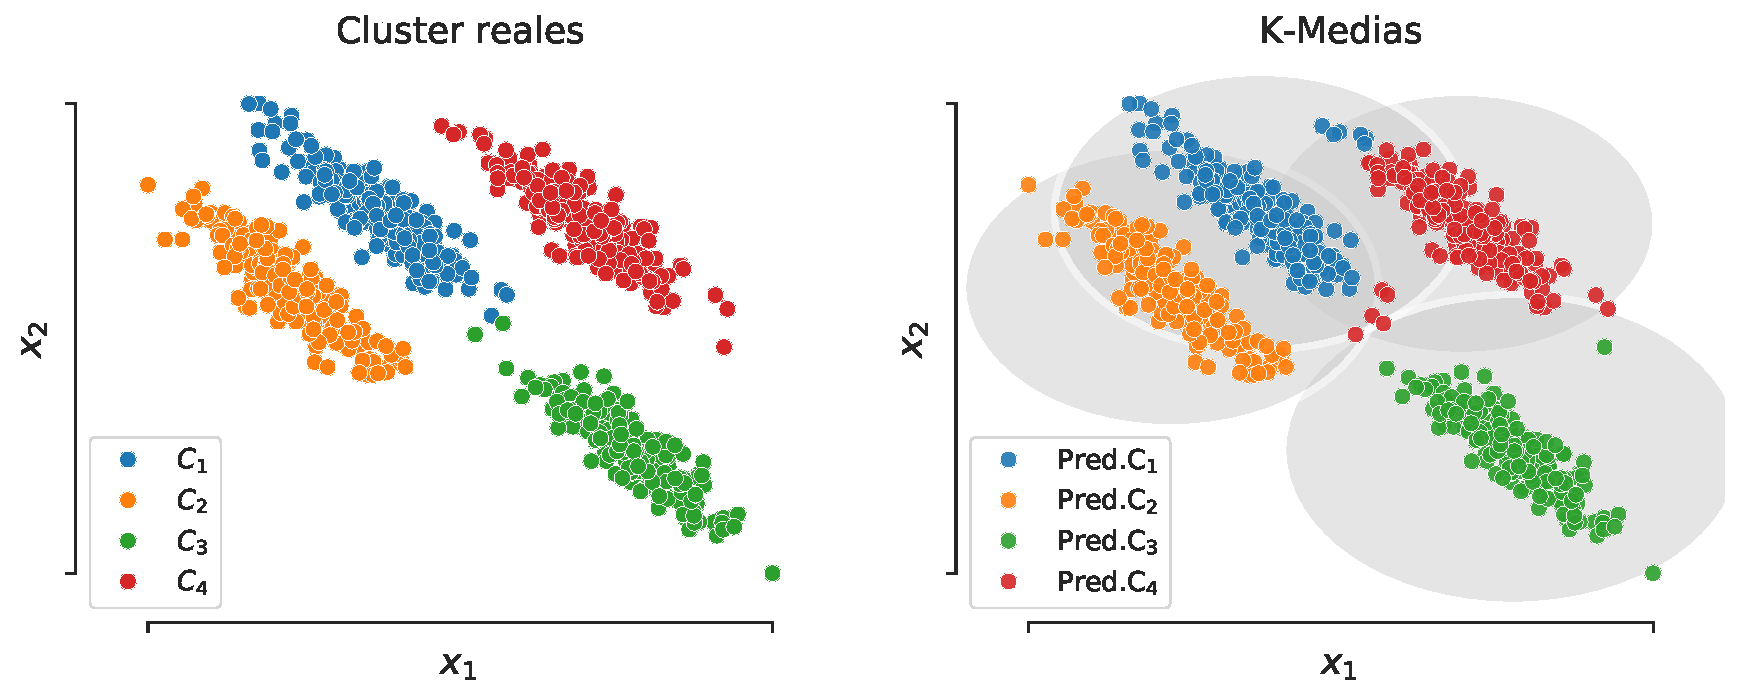
\includegraphics[width=0.8\textwidth]{img/cap7_k_medias}
  \caption{(Izquierda) Datos reales con sus etiquetas correctas. (Derecha) Clusters encontrados por k-means.}
  \label{fig:kmeans}
\end{figure}



\subsection{Modelo de mezcla de gaussianas}

La mezcla de gaussianas (GMM, por su sigla en inglés) es un caso general de k-means, en donde los clusters pueden tener una forma anisotrópica modelada por una Gaussiana con covarianza no necesariamente proporcional a la identidad. Además, si bien su solución puede ser muy similar a K-means los supuestos subyacentes al modelo CMM son diferentes y obedecen a un enfoque de modelo generativo. 

Recordemos que una distribución de mezcla de gaussianas dada por 
\begin{align}
p(\x) = \sum_{k=1}^K \pi_k \mathcal{N}(\xi| \mu_k,\Sigma_k)
\end{align}
es un modelo para aproximar distribuciones mediante la consideración de varias componentes $K\in\N$. Nos referiremos a los parámetros de este modelo como 

\begin{itemize}
	\item $\pi_k:$ coeficiente de mezcla del cluster  $k$
	\item $\mu_k:$ media del cluster  $k$
	\item $\Sigma_k:$ matriz de covarianza del cluster  $k$
\end{itemize}

En el caso de clustering, es necesario además saber de qué componente fue generada cada muestra. Con el mismo criterio que $K$-means, podemos asignar una variable latente, denotada $\z = [z_1,z_2,\ldots,z_K]^\top\in\{0,1\}^K$, que describe la asignación de cada muestra a cada cluster, es decir, $z_{k}=1$ si la observación $x_n$ pertenece al cluster $k$, y $z_{k}=0$ si no. 

Podemos denotar la distribución marginal del cluster $k$, es decir, de que una observación sea generada por la $k$-ésima componente como 
\begin{equation}
 	p(z_k=1) = \pi_k \label{eq:GMM_marg1}
\end{equation} 
con lo que la distribución marginal del vector $\z$ puede expresarse como 
\begin{equation}
	p(\z) = \prod_{k=1}^K \pi_k^{z_k} \label{eq:GMM_marg2}
\end{equation}
pues recordemos que $\sum_{k=1}^K {z_k} =1$ y $\sum_{k=1}^K {\pi_k}=1$. 

Adicionalmente, podemos describir la distribución condicional de $\x$, dado que su componente es la $k$-ésima, i.e., $z_k=1$, como 
\begin{equation}
	p(\x|z_{k}=1) = \cN(\x|\mu_k,\Sigma_k) \label{eq:GMM_cond1}
\end{equation}
y consecuente su distribución condicional como 
\begin{equation}
	p(\x|\z) = \left(\cN(\x|\mu_k,\Sigma_k)\right)^{z_k} \label{eq:GMM_cond2}
\end{equation}
Multiplicando las ecuaciones \eqref{eq:GMM_marg2} y \eqref{eq:GMM_cond2}, podemos obtener la distribución conjunta de $\x$ y $\z$, donde luego sumando  c.r.a. $k$, recuperamos la distribución marginal de $\x$ de suma de gaussianas mediante el uso de la variable latente $\z$. Respectivamente: 
\begin{align}
	p(\x,\z) &= \left(\pi_k\cN(\x|\mu_k,\Sigma_k)\right)^{z_k}\\
	p(\x) 	&= \sum_{k=1}^K p(\x,\z) = \sum_{k=1}^K \pi_k \cN(\x|\mu_k,\Sigma_k)
\end{align}

\begin{mdframed}[style=pendiente, frametitle={\center discusión}]
¿Por qué la conjunta es \emph{mejor} que la marginal?\\
Como generar muestras: ancestral sampling

\end{mdframed}


\subsubsection{Posterior} 
\label{sub:GMM_posterior}

Veamos ahora la forma que toma la distribución posterior de la variable latente $z$, usando el teorema de Bayes, tenemos 

\begin{align}
	p(z_k=1|\x) = \frac{p(\x|z_k=1)p(z_k=1)}{p(\x)} = \frac{\pi_k \cN(\x|\mu_k,\Sigma_k)}{\sum_{k=1}^K \pi_k \cN(\x|\mu_k,\Sigma_k)} \label{eq:GMM_post1}
\end{align}
esta cantidad también se llama \emph{responsabilidad} de la componente $k$ por la observación $\x$.

\subsubsection{Máxima verosimilitud} 
\label{sub:GMM_ml}

Recordemos que los parámetros del modelo de mezcla de gaussianas son los coeficientes de mezcla, las medias y varianzas de cada componente. Si disponemos de un conjunto de observaciones $\{\x_n\}_{n=1}^N$, entonces podemos encontrar dichos parámetros mediante máxima verosimilitud. Observe que la log-verosimilitud está dada por 

\begin{equation}
	\log p(\x_1,\x_2,\ldots,\x_N) = \sum_{n=1}^N \log p(\x_n) = \sum_{n=1}^N \log \sum_{k=1}^K  \pi_k\cN(\x_n|\mu_k,\Sigma_k) \label{eq:GMM_like}	
\end{equation}
Observemos que hay una serie de complicaciones relacionados a la búsqueda de estos parámetros mediante la maximización de las ecuación \eqref{eq:GMM_like}. Primero, están las soluciones dadas por singularidades cuando una muestra es exactamente igual a una de las medias, en cuyo caso un término de la log-verosimilitud es proporcional a $1/\sigma_k$, con lo que la maximización te $\sigma_k$ resulta en una log-verosimilitud infinita. En segundo lugar tenemos las redundancias de soluciones: para cada máximo local (o solución en general) de la log-verosimilitd existen $K!$ soluciones equivalente con la misma verosimilitud dadas por las permutaciones de las etiquetas de los clusters. Finalmente, optimizar la log-verosimilitud de la mezcla de gaussianas es desafiante porque la sumatoria aparece \emph{dentro} del logaritmo, consecuentemente,  el logaritmo no actúa directamente en la gaussiana reduciendo el funcional de optimización a una solución en forma cerrada. Por esta razón, es necesario considerar basados en gradiente.

\begin{mdframed}[style=pendiente, frametitle={\center discusión}]
¿Por qué no hay \emph{singularidades} en el caso de una gaussiana?
\end{mdframed}


\subsubsection{Entrenamiento} 
\label{sub:GMM_train}

Veamos las condiciones de primer orden para encontrar los parámetros, es decir, igualando el gradiente (con respecto a cada uno de los parámetros) de la log-verosimilitud igual a cero. Denotando $\gamma(z_{nk}) = p(z_{nk}=1|\x_n)$, obtenemos

 
    \begin{align}
    \mu_k & = \frac{1}{R_k}\sum_{n=1}^N \gamma(z_{nk})\x_i\\
    \Sigma_k & = \frac{1}{R_k} \sum_{n=1}^N \gamma(z_{nk})(\x_n - \mu_k)(\x_n - \mu_k)^\top\\
    \pi_k & = \frac{R_k}{R},
    \end{align}
    donde
    \begin{align*}
    R_k = \sum_{i=n}^N \gamma(z_{nk}) \qquad \text{y} \qquad R = \sum_{k=1}^K R_k.
    \end{align*}

  Observe que esto no constituye una solución en forma cerrada para los parámetros, pues la posterior $\gamma(z_{nk})$ depende de todos los parámetros de acuerdo a la ecuación \eqref{eq:GMM_post1}. Sin embargo, podemos considerar un procedimiento iterativo en donde calculamos las posteriores $\gamma(z_{nk})$ (llamado paso E), para luego calcular los parámetros óptimos de acuerdo a las ecuaciones anteriores (llamado paso M). 



\underline{\textbf{Ejemplo:}} La figura \ref{fig:gmm} muestra un ejemplo de clustering utilizando GMM. En este caso, se puede observar directamente como GMM es una generalización de kmeans, en donde ahora los clusters tienen forma de gaussiana anisotrópica.

\begin{figure}[ht]
  \centering
  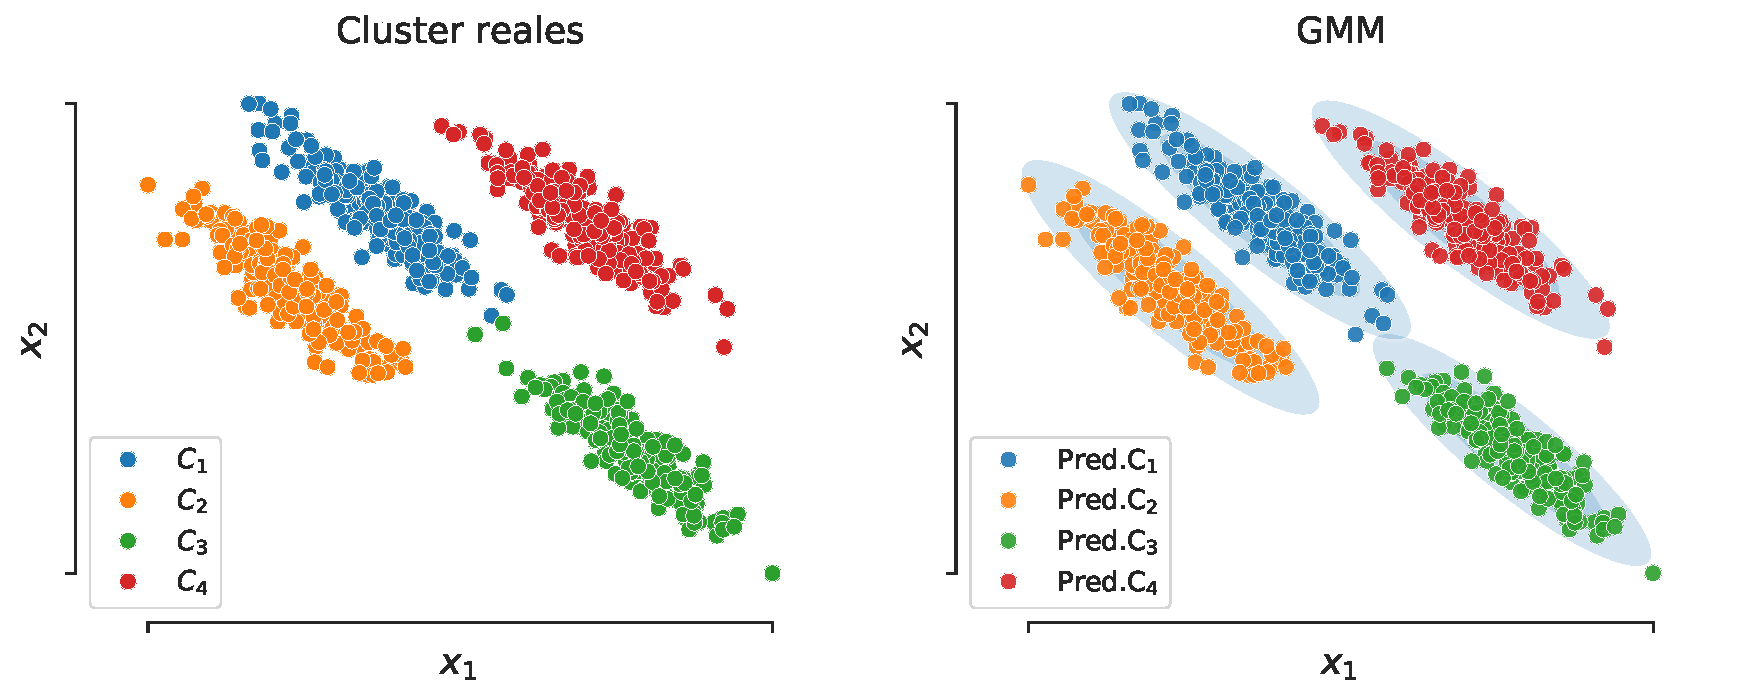
\includegraphics[width=0.8\textwidth]{img/cap7_gmm}
  \caption{(Izquierda) Datos reales con sus etiquetas correctas. (Derecha) Clusters encontrados por GMM.}
  \label{fig:gmm}
\end{figure}



\subsubsection{Expectation-Maximisation} 
\label{sub:GMM_EM}

En el caso general, donde tenemos \emph{observables} $\x$, variables latentes $\z$ y parámetros $\theta$, y un modelo descrito por una distribución marginal que puede ser expresada mediante 

\begin{equation}
	\log p(\x|\theta) = \log \int p(\x,\z|\theta)d\z
\end{equation}
donde tenemos logaritmos de sumas, lo cual es complicado de optimizar, incluso cuando la distribución conjunta $p(\x,\z|\theta)$ está en la familia exponencial.  

Asumamos por un momento que tenemos valores para la variable latente $\z$, si este fuese el caso, podríamos buscar los parámetros mediante la optimización de la log-verosimilitud completa, $\log p(\x, \z |\theta)$, la cual como en GMM puede tener una forma más simple de optimizar debido a que no hay una suma dentro del logaritmo. 

En la práctica, sin embargo, no tenemos acceso al valor de las variables latentes $\z_n$ sino que únicamente podemos acceder a una estimación de éstas mediante la distribución posterior $p(\z|\x,	\theta)$. Entonces, estrictamente hablado, la cantidad que nos gustaría maximizar $\log p(\x, \z |\theta)$ es aleatoria, por lo que podemos maximizar su esperanza con respecto a las observaciones (etapa de Maximización). Luego, con los valores obtenidos para los parámetros podemos recalcular la distribución posterior $p(\z|\x,\theta)$ (etapa de Esperanza) y seguir este proceso iterativamente. La motivación de este procedimiento, llamado \emph{Expectation-Maximisation}, es que en primer lugar, con la cantidad $p(\z|\x,\theta)$ fija, el cálculo de los nuevos parámetros mediante máxima verosimilitud indiscutiblemente aumenta la verosimilitud, luego éstos mejores parámetros dan consecuentemente una mejor estimación de la distribución posterior $p(\z|\x,\theta)$, con lo cual la actualización de los parámetros usando esta mejorada aproximación de la posterior debe ser incluso mejor. 

\begin{mdframed}[style=pendiente, frametitle={\center discusión}]
Bayesian GMM: ¿cómo elegir la cantidad de Gaussianas?
\end{mdframed}




\subsection{Density-based spatial clustering of applications with noise (DBSCAN)}

Es un algoritmo de clustering propuesto por Martin Ester et al. el cual ha tenido mucha popularidad puesto que no requiere definir una cantidad inicial de número de clusters. Los hiper-parámetros de entrada del modelo son 2:

\begin{itemize}
    \item Mínimo número de punto $minPts$.
    \item Radio o vecindad $\epsilon$.
\end{itemize}

El algoritmo se basa en la idea de que dado 2 púntos $x_i$, $x_j$ dentro de un mismo cluster, se dice que \emph{$x_i$ es alcanzable por $x_j$}, si siempre se puede llegar de $x_i$ a $x_j$ avanzando de punto en punto, donde la distancia entre cada uno es al menos menor que $\epsilon$ y además un punto intermedio es un punto núcleo. Con estos el algoritmo define tres tipos de puntos:

\begin{itemize}
    \item \textbf{Puntos núcleo:} Son puntos $x_i$ tales que en una vecindad $\epsilon$ tienen almenos $minPts$ vecinos.
    \item \textbf{Puntos borde:} Constituyen el \textit{borde externo} de los cluster.
    \item \textbf{Outliers:} Puntos que no son alcanzables por ningún punto.
\end{itemize}

Notemos que con lo anterior, se desprende que todo cluster debe tener al menos un punto núcleo.
El algoritmo para encontrar los clusters es el siguiente:


\begin{algorithm}[H]
  \caption{Pseudo código de DBSCAN
    \label{DBSCAN}}
  \begin{algorithmic}[1]
    \Function{DBSCAN}{$D, eps, MinPts$}
      \State $C \gets 0$\;
      \For{{cada punto $P$ no visitado en $D$}}
      \State marcar $P$ como visitado
        \If{sizeOf(PuntosVecinos) $\le$ MinPts}
        \State marcar $P$ como RUIDO
        \Else
        \State C $\gets$ C+1
        \State expandirCluster(P,vecinos, C, eps, MinPts)
        \EndIf
      \EndFor
    \EndFunction
  \end{algorithmic}
\end{algorithm}


\begin{algorithm}[H]
  \caption{Función para expandir cluster.
    \label{alg:expandirCluster}}
  \begin{algorithmic}[1]
  \Function{expandirCluster}{P, vecinosPts, C, eps, MinPts}
  \State agregar P al cluster C
  \For{cada punto P' en vecinosPts}
  \If{P' no fue visitado}
         \State marcar P' como visitado\;
         \State vecinosPts' $\gets$ regionDeConsulta(P', eps)\;
         \If{sizeof(vecinosPts') $\geq$ MinPts}
            \State vecinosPts $\gets$ vecinosPts $\cup$ vecinosPts'
        \EndIf
    \EndIf
    \If{P' no tiene cluster asignado}
         \State P' se le asigna el cluster C
    \EndIf
    \EndFor
    \EndFunction
  \end{algorithmic}
\end{algorithm}


\begin{algorithm}[H]
  \caption{Retorna los puntos de la vecindad de búsqueda para un punto.
    \label{alg:regionDeConsulta}}
  \begin{algorithmic}[1]
    \Function{regionDeConsulta}{$P, eps$}
    
    \Return Todos los puntos junto a P' que están a eps de distancia (incluyendo P)
    \EndFunction
  \end{algorithmic}
\end{algorithm}


\underline{\textbf{Ejemplo:}} La figura \ref{fig:dbscan} muestra un ejemplo de clustering utilizando DBSCAN. La figura \ref{fig:dbscan}(derecha) muestra en negro los puntos que son clasificados como ruido o \emph{outliers} por el algoritmo. Por otro lado, los puntos núcleos son graficados como un punto grande, mientras que los puntos borde se grafican con un marcador pequeño.

\begin{figure}[H]
  \centering
  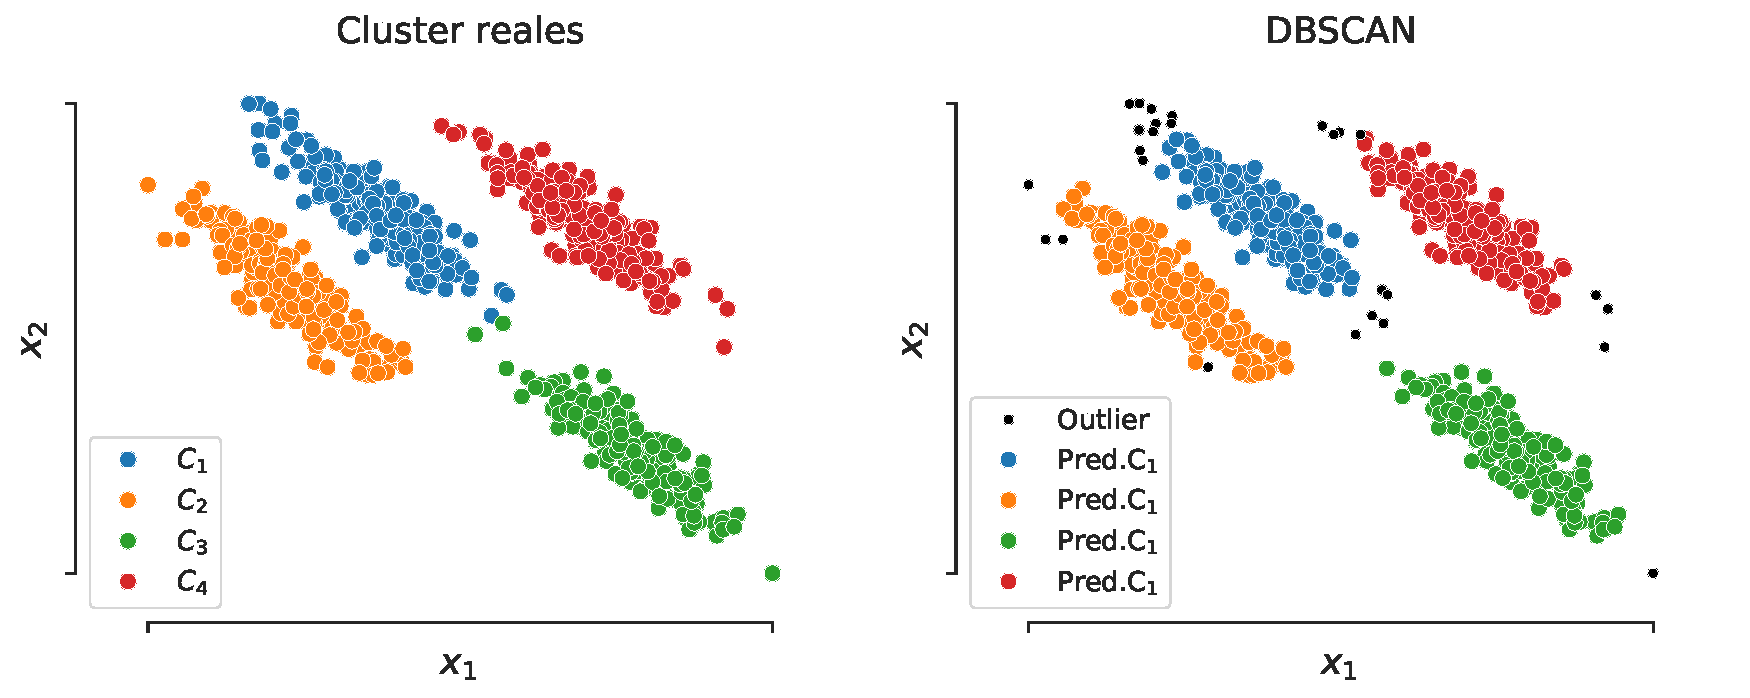
\includegraphics[width=0.8\textwidth]{img/cap7_dbscan}
  \caption{(Izquierda) Datos reales con sus etiquetas correctas. (Derecha) Clusters encontrados por DBSCAN.}
  \label{fig:dbscan}
\end{figure}